% Template for Cogsci submission with R Markdown

% Stuff changed from original Markdown PLOS Template
\documentclass[10pt, letterpaper]{article}

\usepackage{cogsci}
\usepackage{pslatex}
\usepackage{float}
\usepackage{caption}

% amsmath package, useful for mathematical formulas
\usepackage{amsmath}

% amssymb package, useful for mathematical symbols
\usepackage{amssymb}

% hyperref package, useful for hyperlinks
\usepackage{hyperref}

% graphicx package, useful for including eps and pdf graphics
% include graphics with the command \includegraphics
\usepackage{graphicx}

% Sweave(-like)
\usepackage{fancyvrb}
\DefineVerbatimEnvironment{Sinput}{Verbatim}{fontshape=sl}
\DefineVerbatimEnvironment{Soutput}{Verbatim}{}
\DefineVerbatimEnvironment{Scode}{Verbatim}{fontshape=sl}
\newenvironment{Schunk}{}{}
\DefineVerbatimEnvironment{Code}{Verbatim}{}
\DefineVerbatimEnvironment{CodeInput}{Verbatim}{fontshape=sl}
\DefineVerbatimEnvironment{CodeOutput}{Verbatim}{}
\newenvironment{CodeChunk}{}{}

% cite package, to clean up citations in the main text. Do not remove.
\usepackage{cite}

\usepackage{color}

% Use doublespacing - comment out for single spacing
%\usepackage{setspace}
%\doublespacing


% % Text layout
% \topmargin 0.0cm
% \oddsidemargin 0.5cm
% \evensidemargin 0.5cm
% \textwidth 16cm
% \textheight 21cm

\title{Testing the interaction between active and passive learning}


\author{{\large \bf Kyle MacDonald} \\ \texttt{kyle.macdonald@university.edu} \\ Department of Psychology \\ Stanford University \And {\large \bf Michael C. Frank} \\ \texttt{mcfrank@university.edu} \\ Department of Psychology \\ Stanford University}

\begin{document}

\maketitle

\begin{abstract}
In active learning, people have the opportunity to select highly
informative examples based on their current hypotheses, potentially
allowing them to learn faster. But learning contexts often involve
sequences that contain both active and passive learning, an interaction
that we know little about. In the current work, we explore the
interaction between active and passive learning in three category
learrning experiments with adults. First, we replicate the active over
passive learning advantage found in Markant \& Gureckis (2014)
(Experiments 1a and 1b). Then, in Experiments 2 and 3 we provide direct
tests of how different sequences of active/passive training modulate the
effectiveness of active learning in two markedly different concept
learning tasks. Across all three experiments, active training lead to
better learning of the target concept. Passive-first training was more
effective compared to Active-first in both Experiments 2 and 3. Our data
provide evidence that active learning can be more effective once the
learner is given passive experience, providing them with a better
representation of the learning task.

\textbf{Keywords:}
active learning, category learning, replication, order effects
\end{abstract}

\section{Introduction}\label{introduction}

Active learning describes a process where people can select what
information they will learn
next.\footnote{Here we focus on deliberate decisions about what to learn, as opposed to other uses of the term "active" learning (e.g., being engaged with learning materials).}
This context stands in contrast to passive learning, where people
receive information presented to them from the world. For example,
consider a child playing with a new toy, testing to see how it works
(active) compared to a child watching someone else play with the toy
(passive). In both scenarios, the child sees a toy and some of its
functions, but in the active context, the child has control over the
sequence of incoming information.

The potential benefits of active learning have been the focus of
research in education (Grabinger \& Dunlap, 1995), machine learning
(Settles, 2012), and cognitive science (Castro et al., 2009). In their
synthesis of this literature, Gureckis \& Markant (2012) present four
``cognitive'' explanations for why selecting information could improve
learning outcomes: (1) selection of the most informative examples, (2)
increased memory for selected examples, (3) direct knowledge of the
sampling process, and (4) planning an action leads to a deeper
understanding of the task.

In the majority of these studies, researchers isolate active and passive
training sets, and test which regime leads to better learning outcomes.
For example, Markant \& Gureckis (2014) compared the effectiveness of
active vs.~passive training on the rate of participants' learning of two
category structures: a Rule-Based (RB) structure where the category
boundary varied along a single dimension, and and
Information-Integration (II) structure where the category boundary was
defined by a linear combination of two dimensions. In the active
learning condition, learners selected examples from the category;
whereas in passive learning condition, the examples were generated
randomly from the underlying distributions. Markant \& Gureckis (2014)
found that participants in the active condition learned faster and
achieved a higher overall accuracy, but this advantage only held for the
less complex, Rule-Based category.

While it is important to directly compare active and passive training,
real-world learning often involve both. Returning to the example of
learning about a new toy -- the child might see some functions
demonstrated by others and then test for others (or vice versa)
\emph{within} the same learning context. But, we know relatively little
about how different sequences of active/passive learning interact to
affect learning outcomes.

Research in education has asked a similar type of question: How does
varying the order of different teaching methods affect learning? One
illustrative example is the study of \emph{Productive Failure}, where
researchers find that first allowing students to struggle with the task
(typically self-directed problem solving), leads to better uptake of the
subsequent instruction (Westermann \& Rummel, 2012). However, this work
does not directly test how starting with instruction would affect the
quality of the pre-instruction problem solving task.

In comparison, there has been relatively little research in the
cognitive sciences on different sequences of active and passive
learning. In a cross-situational word learning task, Kachergis, Yu, \&
Shiffrin (2013) found that people who received a block of active
learning before passive learning preformed better when asked to recall
the newly learned words. The authors suggest that learners developed
better attentional and memory strategies during the active training,
which transferred to the passive training, boosting their overall
acccuracy. But we do not yet know whether this ``active first''
advantage would generalize to other types of learning tasks.

In the current set of studies, we test how different sequences of
active/passive training affect learning outcomes. In Experiments 1a and
1b, we directly replicate the active learning advantage found in Markant
\& Gureckis (2014). In Experiment 2, we build on our replication data to
show that passive-first training is more effective than active-first. In
Experiment 3, we find the same passive-first advantage in a novel
paradigm where participants learn a more complex, heirarchical category
structure. Together, the data suggest that active learning can provide
an advantage over passive learning, but this advantage depends on the
learners' representation of the task, which can be improved by receiving
(a) more active learning or (b) an initial bout of passive learning.

\begin{CodeChunk}
\captionsetup{width=0.8\textwidth}\begin{figure*}[t]

{\centering 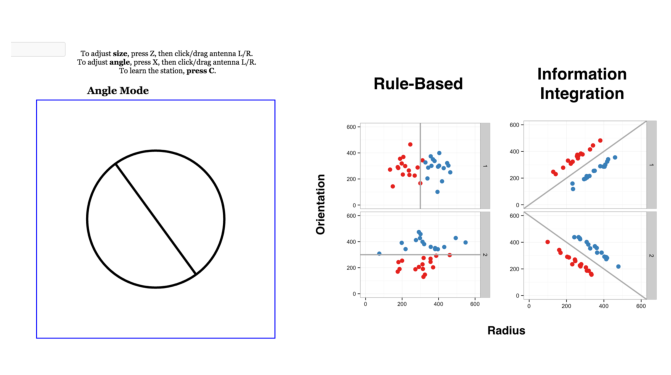
\includegraphics{figs/stimuli_exp1-1} 

}

\caption[The left panel shows a screenshot of the stimuli used in Experiments 1 and 2]{The left panel shows a screenshot of the stimuli used in Experiments 1 and 2. The right panel shows examples of distributions of training stimuli shown to participants passive learning condition from the Rule-Based category and the Information-Integration category.}\label{fig:stimuli_exp1}
\end{figure*}
\end{CodeChunk}

\section{Experiment 1a}\label{experiment-1a}

Experiment 1a is a direct replication of the advantage for active
learning over passive learning found in Markant \& Gureckis (2014). We
tested participants' category learning for the RB category structure
after receiving either active or passive training. We used the same
stimuli and followed the exact procedures as the original study
(described below). All of the stimuli and the experiments can be viewed
and downloaded at the project page for this paper:
\url{https://kemacdonald.github.io/Act-Learn/}.

\begin{CodeChunk}
\captionsetup{width=0.8\textwidth}\begin{figure*}[t]

{\centering 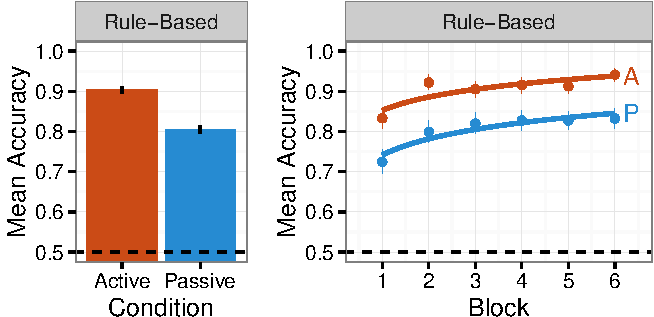
\includegraphics{figs/exp1a_acc_plot-1} 

}

\caption[The left panel shows overall accuracy performance for the Active and Passive training conditions]{The left panel shows overall accuracy performance for the Active and Passive training conditions. The right panel shows participants' accuracy across each of the six blocks in the experiment. Colored lines are generated by a binomial smoother and error bars indicate 95\% confidence intervals computed by non-parametric bootstrap.}\label{fig:exp1a_acc_plot}
\end{figure*}
\end{CodeChunk}

\subsection{Methods}\label{methods}

\subsubsection{Participants}\label{participants}

We posted a set of Human Intelligence Tasks (HITs) to Amazon Mechanical
Turk. Only participants with US IP addresses and a task approval rate
above 85\% were allowed to participate, and each HIT paid one dollar. 53
HITs were posted for each of the two between-subjects conditions. Data
were excluded if participants completed the task more than once or if
they reported that they did not understand the task at the end of the
experiment (1 HITs). The final sample consisted of 52 participants.

\subsubsection{Stimuli}\label{stimuli}

The left panel of Figure 1 shows a screenshot of the stimuli used in
Experiments 1a, 1b, and 2. Visual stimuli were black ``antennas'' on a
white background. Each antenna could vary along two continuous
dimensions -- radius size or central angle -- and was assigned a value
between 1 and 600. These values were converted to pixel values for
display on a computer screen. To ensure that participants could not
complete a full rotation of the antenna, the rotation of the central
angle was limited to 150 degrees. The minimum radius and angle values
were randomized for each participant, such that each participant was
assigned a unique optimal decision boundary. Finally, we used a
Rule-Based category structure where the category boundary is defined
along a single dimension: either the antenna's size or central angle
(see right panel of Figure 1).

Radius and angle values for the 96 passive training trials were
generated from two Gaussian distributions with identical mean and
covariance parameters as Markant \& Gureckis (2014) (see the right panel
of Figure 1). For test trials, we created a uniform grid of 192 unique
test items that covered the entire feature space. We randomly sampled 8
items from each quadrant to get 32 test trials for each block. We then
randomized the order of the training and test trials within each block
for each participant.

\subsubsection{Design and procedure}\label{design-and-procedure}

Participants saw a total of 288 trials (96 training trials and 192 test
trials) across 6 blocks. Each block consisted of 16 training trials and
32 test trials. Before starting the task, participants were told that
this was a game where they would see ``loop antennas'' for televisions
and each antenna received one of two channels (CH1 or CH2), and their
goal was to learn the difference between the two types of antennas. We
introduced some uncertainty by telling participants that the antennas
could pick up the wrong channel on occasion, and that they should learn
what channel is most often received by a particular type of antenna.

After the instructions, participants were randomly assigned to one the
two between-subjects conditions (Active vs.~Passive training). In the
Active training condition, participants were able to design their own
antennas to test. They modified the antenna by clicking and dragging the
mouse from left to right. To change the size of the antenna, they first
pressed the ``Z'' key. To change the angle, they first pressed the ``X''
key. When participants were finished with their design, they pressed the
spacebar to see which channel (Ch1 or Ch2) the antenna received. The
channel label appeared in a text box with a green border located above
the antenna.

In the Passive training condition, participants were shown antennas with
size and angles generated from the underlying category distributions.
After a two second delay they were told which channel the antenna
received. To ensure that participants saw the channel, they had to click
on the channel text in order to advance the experiment. When they
clicked the channel text, a green box appeared around the text to
indicate that their response had been recorded.

After completing the training, participants in both conditions proceeded
to the test trials. On each test trial participants saw an antenna and
were asked, ``Which channel does this antenna receive?'' To indicate
their response participants selected one of two buttons located above
the antenna.

\subsection{Results and Discussion}\label{results-and-discussion}

\subsubsection{Overall classification
accuracy}\label{overall-classification-accuracy}

First, we directly follow the analysis plan of Markant \& Gureckis
(2014), using a t-test to directly compare overall test performance for
participants in the active and passive learning conditions. All of our
data, processing, and analysis code can be viewed in the version control
repository for this paper at:
\texttt{https://github.com/kemacdonald/act-learn}. The left panel of
Figure 2 shows overall test performance, with active learners being more
accurate than passive learners, \(t\)(51) = 2.52, \(p\) = 0.015.

\subsubsection{Classification accuracy across
blocks}\label{classification-accuracy-across-blocks}

The right panel of Figure 2 shows participants' accuracies across blocks
in the experiment. To quantify participants' behavior, we use mixed
effects regression models with the maximal random effects structure
justified by our experimental design: by-subject intercepts. All
mixed-effects models were fit using the lme4 package in R (Bates,
Maechler, Bolker, \& Walker, 2013). We fit a logistic regression
predicting test performance based on condition (active/passive) and
block. The model was specified as
\texttt{Correct $\sim$ 1 + Condition * Block + (1 | subject)}. We found
a significant main effect of condition (\(\beta\) = -0.7, p \textless{}
.001) with better performance for active learners, and significant main
effect of block (\(\beta\) = 0.2, p \textless{} .001) such that
responses were more accurate as the number of blocks increased.

\subsubsection{Relationship between sampling behavior and
learning}\label{relationship-between-sampling-behavior-and-learning}

We were also interested in the relationship between participants'
overall sampling behavior and learning outcomes. We follow
\&markant2014better and quantify the quality of a sample based on it's
orthogonal distance from the true category boundary, with samples closer
to the boundary being of higher quality. For each participant, we
computed a mean accuracy score and a mean sample distance score, and fit
a linear model using sample distance to predict accuracy. We found a
signficant effect of sample distance (\(\beta\) = -.0003, p \textless{}
.001) with accuracy increasing as mean sample distance decreased.

Taken together, our data provide strong evidence for a successful
replication of the original results reported in Markant \& Gureckis
(2014). We found a comparable advantage in overall classification
accuracy for active learners over receptive learners in a web-based
experiment with two fewer training/test trial blocks. Our results differ
from the original study in that we found an immediate advantage for
active learners after the first block that was not present in the
original study. Next we attempt to replicate Markant \& Gureckis
(2014)'s findings for the II category structure and for the yoked
passive learning condition.

\section{Experiment 1b}\label{experiment-1b}

The goals of Experiment 1b are to (a) replicate Markant \& Gureckis
(2014)'s findings for the more difficult II category structure, and (b)
replicate their finding that passive learners did not benefit from being
``yoked'' to active learner's
data.\footnote{Yoked designs are important because they help dissociate the effects of selection from the effects of seeing better data.}
They did not find an active learning advantage for the II category
structure and yoked learners were worse than active learners even though
they had seen the exact same learning information. We used the same
stimuli and followed the exact procedures as the original study
(described below). However, we reduced the length of the experiment to
two blocks. We made this decision based on finding an immediate active
learning advantage in Experiment 1a.

\subsection{Methods}\label{methods-1}

\subsubsection{Stimuli}\label{stimuli-1}

Visual stimuli were identical to Experiment 1a. We use both the RB
category from Experiment 1a, and we add the II category. The II category
boundary is defined by a linear combination of the size and angle
dimensions (see right panel of Figure 1).

\subsubsection{Participants}\label{participants-1}

Participant recruitment and inclusionary/exclusionary criteria were
identical to those of Experiment 1a (excluded No, 3 HITs). 196 HITs were
posted across each of the category structures (II and RB) and training
conditions (Active, Passive, and Yoked).

\subsubsection{Design and procedure}\label{design-and-procedure-1}

Procedures were identical to those of Experiment 1a. We added a
``yoked'' learning condition, in which we match each passive learning
participant with training data generated from an active learning
participant's sampling behavior. Thus, both the active and yoked
participants saw the exact same data, but the active participants were
in control of the information flow.

\subsection{Results and Discussion}\label{results-and-discussion-1}

\begin{CodeChunk}
\captionsetup{width=0.8\columnwidth}\begin{figure}[t]

{\centering 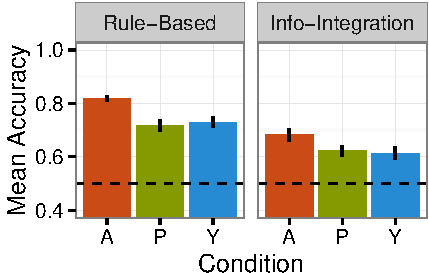
\includegraphics{figs/rep1b-acc-plot-1} 

}

\caption[The left panel shows overall accuracy performance for the Active and Passive training conditions]{The left panel shows overall accuracy performance for the Active and Passive training conditions. The right panel shows participants' accuracy across all six blocks in the experiment.}\label{fig:rep1b-acc-plot}
\end{figure}
\end{CodeChunk}

\subsubsection{Relationship between sampling and test across
blocks}\label{relationship-between-sampling-and-test-across-blocks}

\begin{CodeChunk}
\captionsetup{width=0.8\columnwidth}\begin{figure}[h]

{\centering 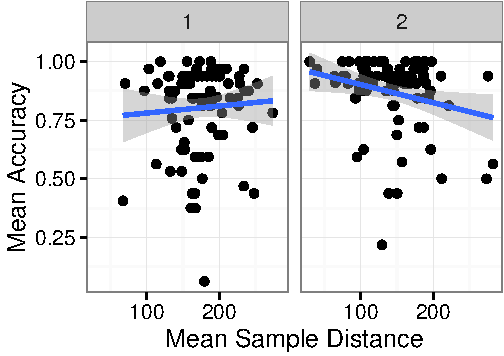
\includegraphics{figs/exp1_sampling-acc-plot-1} 

}

\caption[The relations between quality of sampling and accuracy on test trials across blocks]{The relations between quality of sampling and accuracy on test trials across blocks.}\label{fig:exp1_sampling-acc-plot}
\end{figure}
\end{CodeChunk}

\section{Experiment 2}\label{experiment-2}

\subsection{Methods}\label{methods-2}

\subsubsection{Stimuli}\label{stimuli-2}

Stimuli were identical to Experiment 1.

\subsubsection{Participants}\label{participants-2}

Participant recruitment and inclusionary/exclusionary criteria were
identical to those of Experiment 1 (No, 3 HITs). Approximately 44 HITs
were posted for each condition for total of 176 paid HITs.

\subsubsection{Design and procedure}\label{design-and-procedure-2}

\subsection{Results and Discussion}\label{results-and-discussion-2}

\begin{CodeChunk}
\captionsetup{width=0.8\textwidth}\begin{figure*}[h]

{\centering 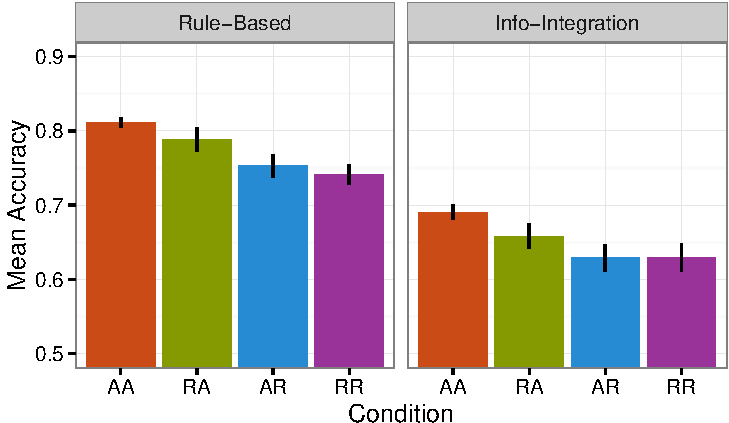
\includegraphics{figs/exp2_acc_plot-1} 

}

\caption[The left panel shows accuracy performance across both blocks for the different sequence of active/passive training]{The left panel shows accuracy performance across both blocks for the different sequence of active/passive training. The right panel shows overall accuracy performance plotted with the active-active and receptive-receptive data from Experiment 1.}\label{fig:exp2_acc_plot}
\end{figure*}
\end{CodeChunk}

\section{Experiment 3}\label{experiment-3}

Experiment 3 is a conceptual replication of the order effect findings
using a novel paradigm where participants learn a higher dimensional
concept.

\subsection{Methods}\label{methods-3}

\subsubsection{Stimuli}\label{stimuli-3}

\subsubsection{Participants}\label{participants-3}

Participant recruitment, and inclusionary/exclusionary criteria were
identical to those of Experiment 1 and 2 (excluded TODO HITs). 40 HITs
were posted for each condition (TODO) for total of TODO paid HITs.

\subsubsection{Design and procedure}\label{design-and-procedure-3}

\subsection{Results and Discussion}\label{results-and-discussion-3}

\begin{table}[H]
\centering
\begin{tabular}{rrrrr}
  \hline
 & Estimate & Std. Error & t value & Pr($>$$|$t$|$) \\ 
  \hline
(Intercept) & -0.07 & 0.09 & -0.7 & 0.46 \\ 
  x & 1.98 & 0.09 & 23.3 & 0.00 \\ 
   \hline
\end{tabular}
\end{table}

\section{General Discussion}\label{general-discussion}

\begin{itemize}
\itemsep1pt\parskip0pt\parsep0pt
\item
  Recap findings

  \begin{itemize}
  \itemsep1pt\parskip0pt\parsep0pt
  \item
    Active learning advantage in a direct replication (yay science!)
  \item
    Passive-active better than Active-passive
  \item
    Conceptual replication
  \end{itemize}
\item
  Expand on why we see AR \textgreater{} RA

  \begin{itemize}
  \itemsep1pt\parskip0pt\parsep0pt
  \item
    Sequential hypothesis testing model
  \item
    Gain some understanding of task before exploring
  \item
    RA is bad because you can't refine your current hypothesis. Can only
    use the data you are given to confirm/reject current hypothesis
  \end{itemize}
\item
  Limitations

  \begin{itemize}
  \itemsep1pt\parskip0pt\parsep0pt
  \item
    AA was always best
  \item
    task analysis
  \item
    complexity of real world learning
  \end{itemize}
\item
  Takeaway point:
\end{itemize}

\section{Acknowledgements}\label{acknowledgements}

We are grateful to Doug Markant and Todd Gureckis for sharing the
details and code from the original experiment. We thank the members of
the Language and Cognition Lab for their helpful feedback on this
project. This work was supported by a National Science Foundation
Graduate Research Fellowship to KM.

\section{References}\label{references}

\setlength{\parindent}{-0.1in} \setlength{\leftskip}{0.125in} \noindent

Bates, D., Maechler, M., Bolker, B., \& Walker, S. (2013). Lme4: Linear
mixed-effects models using eigen and s4. \emph{R Package Version},
\emph{1}(4).

Castro, R. M., Kalish, C., Nowak, R., Qian, R., Rogers, T., \& Zhu, X.
(2009). Human active learning. In \emph{Advances in neural information
processing systems} (pp. 241--248).

Grabinger, R. S., \& Dunlap, J. C. (1995). Rich environments for active
learning: A definition. \emph{Research in Learning Technology},
\emph{3}(2).

Gureckis, T. M., \& Markant, D. B. (2012). Self-directed learning a
cognitive and computational perspective. \emph{Perspectives on
Psychological Science}, \emph{7}(5), 464--481.

Kachergis, G., Yu, C., \& Shiffrin, R. M. (2013). Actively learning
object names across ambiguous situations. \emph{Topics in Cognitive
Science}, \emph{5}(1), 200--213.

Markant, D. B., \& Gureckis, T. M. (2014). Is it better to select or to
receive? Learning via active and passive hypothesis testing.
\emph{Journal of Experimental Psychology: General}, \emph{143}(1), 94.

Settles, B. (2012). Active learning. \emph{Synthesis Lectures on
Artificial Intelligence and Machine Learning}, \emph{6}(1), 1--114.

Westermann, K., \& Rummel, N. (2012). Delaying instruction: Evidence
from a study in a university relearning setting. \emph{Instructional
Science}, \emph{40}(4), 673--689.

\end{document}
